%% LyX 2.3.6 created this file.  For more info, see http://www.lyx.org/.
%% Do not edit unless you really know what you are doing.
\documentclass[english,aspectratio=169]{beamer}
\usepackage{lmodern}
\renewcommand{\sfdefault}{lmss}
\renewcommand{\ttdefault}{lmtt}
\usepackage[T1]{fontenc}
\usepackage[latin9]{inputenc}
\setlength{\parskip}{\medskipamount}
\setlength{\parindent}{0pt}
\usepackage{amstext}
\usepackage{amssymb}
\usepackage{graphicx}

\makeatletter

%%%%%%%%%%%%%%%%%%%%%%%%%%%%%% LyX specific LaTeX commands.
\pdfpageheight\paperheight
\pdfpagewidth\paperwidth


%%%%%%%%%%%%%%%%%%%%%%%%%%%%%% Textclass specific LaTeX commands.
% this default might be overridden by plain title style
\newcommand\makebeamertitle{\frame{\maketitle}}%
% (ERT) argument for the TOC
\AtBeginDocument{%
  \let\origtableofcontents=\tableofcontents
  \def\tableofcontents{\@ifnextchar[{\origtableofcontents}{\gobbletableofcontents}}
  \def\gobbletableofcontents#1{\origtableofcontents}
}

%%%%%%%%%%%%%%%%%%%%%%%%%%%%%% User specified LaTeX commands.
\usetheme{AnnArbor}
\usecolortheme{seagull}
\hypersetup{}
\usepackage{tikz}
\usepackage{color}
\usepackage{listings}

\makeatother

\usepackage{babel}
\begin{document}
\title[M7-1]{The thermal wind}
\author{Department of Oceanography}
\institute[UCT]{University of Cape Town}
\date{SEA3004F}
\makebeamertitle

\section*{Outlines}
\begin{frame}{Outline}

\tableofcontents{}
\end{frame}


\section{Barotropic and baroclinic conditions}
\begin{frame}{The Gulf Stream: vertical structure of temperature}
\begin{center}
\includegraphics[width=0.85\paperwidth]{figures/M7/Gulf_stream}
\par\end{center}

\end{frame}
%
\begin{frame}{The Northern Benguela current: vertical structure of temperature}
\begin{center}
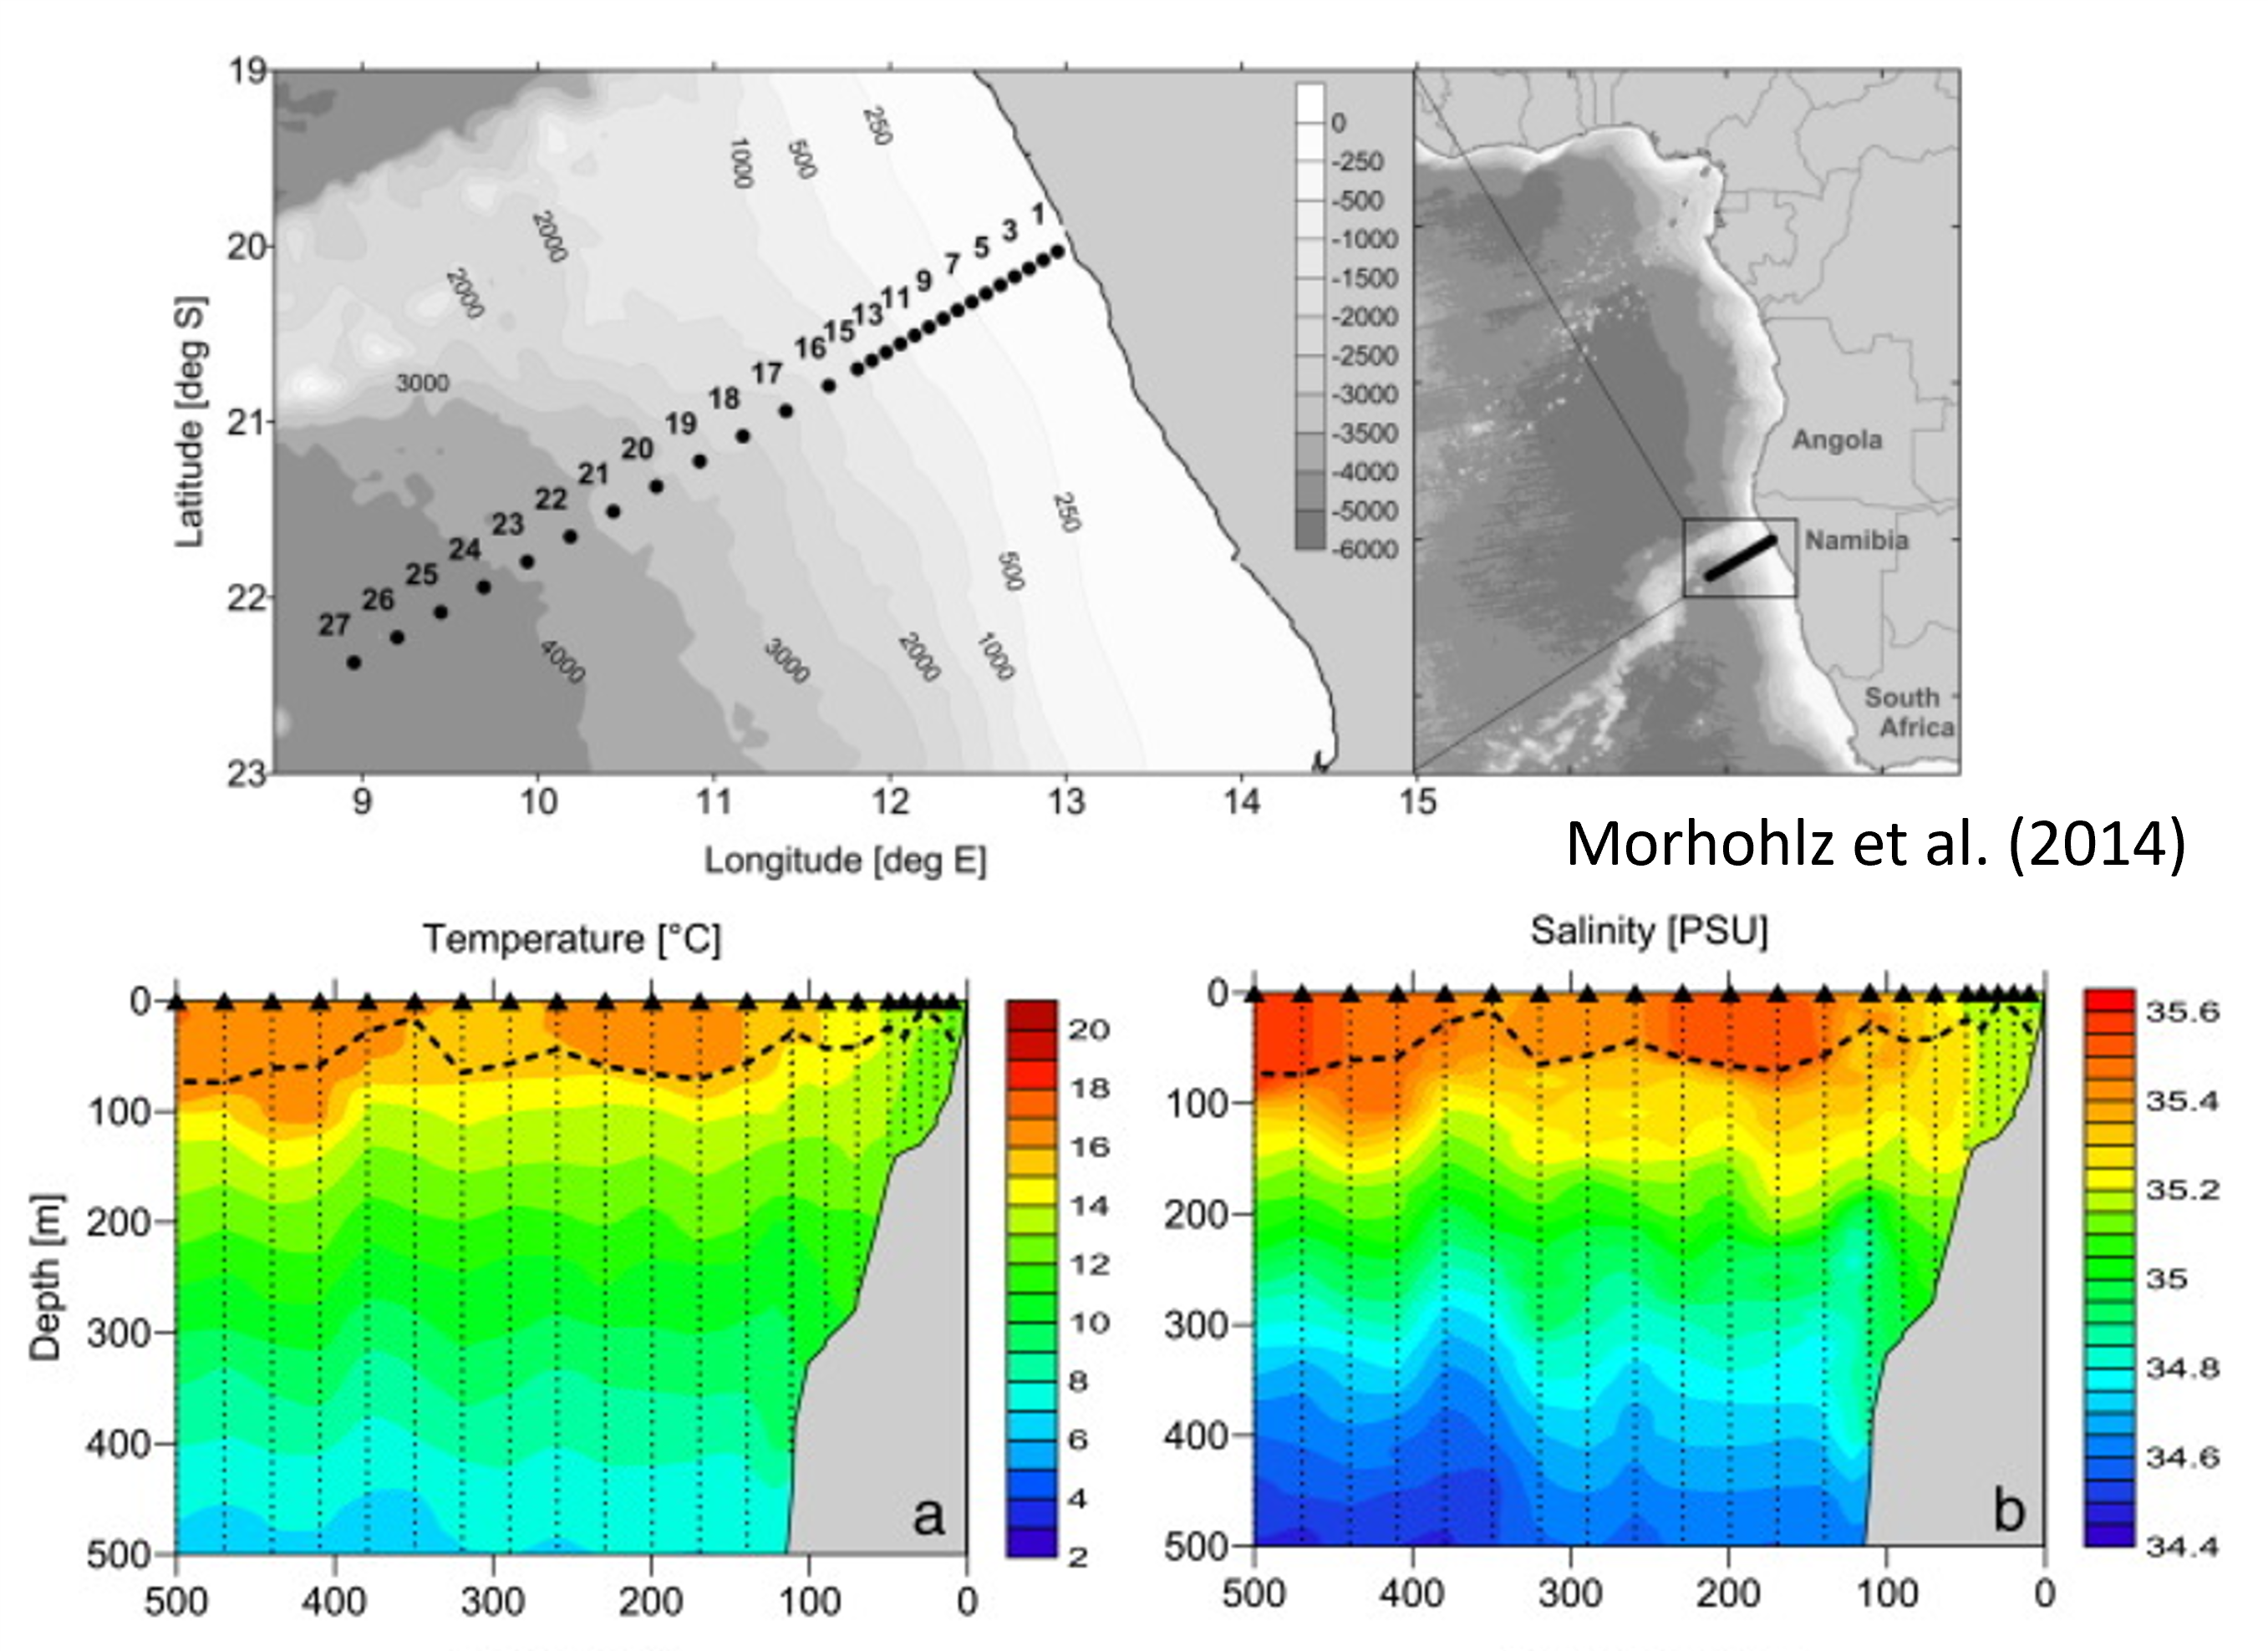
\includegraphics[width=0.55\paperwidth]{figures/M7/Agulhas_temperature}
\par\end{center}

\end{frame}
%
\begin{frame}{Barotropic and baroclinic conditions}

\begin{center}
\includegraphics[width=10cm]{figures/M7/barotropic_baroclinic}
\par\end{center}
\begin{itemize}
\item {\tiny{}Our idealized ocean has constant density and }\textbf{\tiny{}isobaric
surfaces}{\tiny{} (equal pressure surfaces) parallel to the sea surface
(see Ocean Circulation, 3.3.2). }{\tiny\par}
\item {\tiny{}In the real ocean, density increases with depth because of
the compression due to the increasing weight of the water. Therefore
also the surfaces of equal density are parallel to the sea surface,
called }\textbf{\tiny{}isopycnic or isopycnal surfaces}{\tiny{}. This
conditions are called barotropic (pressure in all places) to indicate
that pressure gradients are equal at any depth. }{\tiny\par}
\item {\tiny{}We know that density is affected by variations in temperature
(heat fluxes) and salinity (freshwater fluxes). The isopycnals do
not follow the sea surface because density is not just driven by pressure.
These differences in density will in turn affect pressure and thus
change the shape of the isobars that will become flattened (on the
right in this example, where water is denser). This conditions, rather
normal in the ocean, are called baroclinic (inclined pressure) to
indicate that isopycnals and isobars are not parallel and cross each
other}{\tiny\par}
\end{itemize}
\end{frame}
%

\section{The Taylor columns}
\begin{frame}{The geostrophic balance}

\begin{center}
\includegraphics[width=5cm]{figures/M7/f07-01-P558691}
\par\end{center}
\begin{itemize}
\item {\footnotesize{}Before starting, we recall the formulation of the
geostrophic wind or current from the previous lectures:
\begin{align}
\mathbf{u}_{g} & =\frac{1}{f\rho_{0}}\hat{\mathbf{k}}\times\nabla_{H}p\nonumber \\
\left\langle u_{g},v_{g}\right\rangle  & =\left\langle -\frac{1}{f\rho_{0}}\frac{\partial p}{\partial y},\frac{1}{f\rho_{0}}\frac{\partial p}{\partial x}\right\rangle \label{eq:geostrophic}
\end{align}
}{\footnotesize\par}
\end{itemize}
\end{frame}

\begin{frame}{Taylor columns}

\begin{columns}

\column{7cm}

\centering\includegraphics[scale=0.2]{figures/M7/f07-07-P558691}
\begin{itemize}
\item {\scriptsize{}The experiment with the rotating tank shows that a fluid
in solid body rotation develops a peculiar circulation characterized
by vertical curtains that maintain the colours of the dye separate.
The figure above shows the difference between a non-rotating and a
rotating experiment. }{\scriptsize\par}
\item {\scriptsize{}The motion is homogeneous in the vertical as if the
water was solid and when an obstacle is encountered, the fluid behaves
as a rigid column, passing around it. These phenomena are called }\textbf{\scriptsize{}Taylor
columns}{\scriptsize\par}
\end{itemize}

\column{6cm}

{\scriptsize{}From the geostrophic balance equation, we can see that
the geostrophic flow in a }\textbf{\scriptsize{}barotropic fluid}{\scriptsize{}
indeed does not have a vertical variation. This is quickly demonstrated
if we assume homogenous density $\rho_{0}$ and compute the vertical
derivative of eq. (\ref{eq:geostrophic}):
\[
\frac{\partial u_{g}}{\partial z}=-\frac{1}{f\rho_{0}}\frac{\partial}{\partial y}\frac{\partial p}{\partial z}=-\frac{1}{f\rho_{0}}\frac{\partial}{\partial y}\left(-\rho_{0}g\right)=0
\]
\[
\frac{\partial v_{g}}{\partial z}=\frac{1}{f\rho_{0}}\frac{\partial}{\partial x}\frac{\partial p}{\partial z}=-\frac{1}{f\rho_{0}}\frac{\partial}{\partial x}\left(-\rho_{0}g\right)=0
\]
Note that we can swap the derivatives since they are linear operators,
and that we have substituted the hydrostatic equilibrium to develop
the vertical pressure gradient.}{\scriptsize\par}
\end{columns}

\end{frame}

\begin{frame}{A more rigorous derivation: the Taylor-Proudman theorem}

\begin{columns}[t]


\column{7cm}
\begin{itemize}
\item {\scriptsize{}We take the general momentum equation in the case of
frictionless flow at low Rossby number (the vertical axis is now directed
along $\mathbf{\Omega}$) }\textrm{\scriptsize{}
\[
0=\underbrace{-\frac{\nabla p}{\rho}}_{\textrm{Pressure gradient}}\underbrace{-2\Omega\times\mathbf{u}}_{\textrm{Coriolis}}\underbrace{-\nabla\phi}_{\textrm{Geopotential}}
\]
}{\scriptsize{}and then compute the curl of all terms to make use
of the property that the curl of a gradient is 0. (see the accompanying
video and M\&P)}{\scriptsize\par}
\item {\scriptsize{}We have to solve the curl of a vector product, similar
to $\mathbf{a}\times\left(\mathbf{b}\times\mathbf{c}\right)=\mathbf{b}\mathbf{\left(a\cdot\mathbf{c}\right)-}\mathbf{c}\mathbf{\left(a\cdot\mathbf{b}\right)}$
but since there is the operator $\nabla$, the derivative of the product
returns more terms:
\[
2\Omega\left(\nabla\cdot\mathbf{u}\right)-2\mathbf{u}\left(\nabla\cdot\Omega\right)+2\left(\mathbf{u}\cdot\nabla\Omega\right)-2\left(\Omega\cdot\nabla\mathbf{u}\right)=0
\]
}{\scriptsize\par}
\end{itemize}

\column{7cm}
\begin{center}
\includegraphics[width=3.5cm]{figures/M7/f07-08-P558691}
\par\end{center}

{\scriptsize{}Considering that $\Omega$ is constant and that the
fluid is incompressible, we are left with the property that the velocity
along the direction of $\Omega$ (in this case $z$) does not change
in space, i.e. the flow is 2-dimensional and the flow is }\emph{\scriptsize{}``made
stiff in the direction of $\Omega$''}{\scriptsize{}
\[
\frac{\partial\mathbf{u}}{\partial z}=0
\]
}{\scriptsize\par}
\end{columns}

\end{frame}


\section{The thermal wind}
\begin{frame}{The Gulf Stream: vertical structure of along-stream velocity}
\begin{center}
\includegraphics[width=0.85\paperwidth]{figures/M7/Gulf_stream_velocity}
\par\end{center}

\end{frame}
%
\begin{frame}{Geostrophy with depth: western boundary currents}

\begin{columns}[c]


\column{8cm}

\includegraphics[width=8cm]{figures/M7/Agulhas_velocity_ASCA}

\includegraphics[width=4cm]{figures/M7/ASCA_mooring_diagram}

\column{4cm}

\textbf{\footnotesize{}Southern hemisphere geostrophic flow using
observations:}{\footnotesize{} }\textbf{\footnotesize{}dense waters
on the right of the flow}{\footnotesize{}.}{\footnotesize\par}

{\footnotesize{}Vertical velocity section across the Agulhas current
from the ASCA moorings. The geostrophic current decreases with depth}{\footnotesize\par}
\end{columns}

\end{frame}

\begin{frame}{The Benguela current velocity structure}
\begin{center}
\includegraphics[width=7cm]{figures/M7/Benguela_current_inversion}
\par\end{center}

\end{frame}
%
\begin{frame}{The SH subtropical jet}
\begin{center}
\includegraphics[width=1\paperheight]{figures/M7/SH_subtropical_jet}
\par\end{center}

\end{frame}

\begin{frame}{Geostrophy does vary with height and depth!}

\begin{columns}[t]


\column{7cm}

\includegraphics[width=5cm]{figures/M7/f05-14-P558691.jpg}

{\scriptsize{}We know from the study of geopotential height that isobaric
surfaces slope down from equator to pole. These slopes increase with
height, which implies that the geostrophic wind should increase. Our
previous manipulation of the equations assuming barotropic flow (the
Taylor-Proudman theorem) suggests that geostrophic flow is instead
``rigid`` in the vertical}{\scriptsize\par}

\column{8cm}
\begin{itemize}
\item {\footnotesize{}Why the geostrophic wind changes with height? Does
the non-uniform stratification (baroclinic flow) affect the wind and
current intensity?}{\footnotesize\par}
\item {\footnotesize{}To verify this, we take the x-component of eq. (\ref{eq:geostrophic})
$u_{g}=-\frac{1}{f\rho}\frac{\partial p}{\partial y}$ and we compute
the vertical derivative making use of the hydrostatic balance $\frac{\partial p}{\partial z}=-\rho g$
but now with density not constant: 
\begin{align*}
\frac{\partial}{\partial z}u_{g}= & -\frac{1}{f\rho}\frac{\partial}{\partial y}\frac{\partial p}{\partial z}=\\
= & -\frac{1}{f\rho}\frac{\partial\left(-\rho g\right)}{\partial y}=\frac{g}{f\rho}\frac{\partial\rho}{\partial y}
\end{align*}
\begin{equation}
\left\langle \frac{\partial u_{g}}{\partial z},\frac{\partial v_{g}}{\partial z}\right\rangle =\left\langle \frac{g}{f\rho}\frac{\partial\rho}{\partial y},-\frac{g}{f\rho}\frac{\partial\rho}{\partial x}\right\rangle \label{eq:thermal_wind}
\end{equation}
}{\footnotesize\par}
\end{itemize}
\end{columns}

\end{frame}

\begin{frame}{Reminder: The linear equation of state for seawater}

\begin{columns}[t]


\column{9cm}
\begin{itemize}
\item {\footnotesize{}In the narrow range of T and S found in the ocean,
temperature influences density much more than salinity}{\footnotesize\par}
\item {\footnotesize{}The thermal expansion coefficient is not a constant
and depends on temperature and pressure (and salinity); the mean value
is $100\times10^{-6}$ K$^{-1}$ and it is defined as 
\[
\alpha_{T}=-\frac{1}{\rho_{ref}}\frac{\partial\rho}{\partial T}
\]
}{\footnotesize\par}
\item {\footnotesize{}The haline contraction coefficient gives the change
in density per units salinity (using PSS-78) and has a mean value
of $760\times10^{-6}$ psu$^{-1}$, 
\[
\beta_{S}=\frac{1}{\rho_{ref}}\frac{\partial\rho}{\partial S_{P}}
\]
}{\footnotesize\par}
\item {\footnotesize{}The approximated linear equation of state is a Taylor
expansion around $\sigma_{0}(T_{0},S_{0})$
\[
\sigma=\sigma_{0}+\rho_{ref}\left[-\alpha_{T}\left(T-T_{0}\right)+\beta_{S}\left(S-S_{0}\right)\right]
\]
}{\footnotesize\par}
\end{itemize}

\column{5cm}

\includegraphics[width=4cm]{figures/M7/MP_T94}
\end{columns}

\end{frame}

\begin{frame}{The thermal ``wind''}

\begin{itemize}
\item {\scriptsize{}Eq. (\ref{eq:thermal_wind}) tells us that if density
varies in the horizontal, then the geostrophic current must change
in the vertical. This is the reason why boundary currents in the ocean
usually vanish into a reversed current at depth. The vector form of
the equation is:
\[
\boxed{\frac{\partial\mathbf{u}_{g}}{\partial z}=-\frac{g}{f\rho}\hat{\mathbf{k}}\times\nabla_{H}\rho}
\]
}{\scriptsize\par}
\item {\scriptsize{}This relationship was first demonstrated for the atmosphere,
where the major contributor to density is temperature. This is why
it is termed the}\textbf{\scriptsize{} thermal wind equation}{\scriptsize{}.To
express things in terms of temperature in the ocean, and hence derive
a connection between the current and the thermal field, we can use
the thermal part of the linear equation of state, neglecting salinity
(see next slide for a reminder). We can approximate the density gradient
with the temperature gradient $\left(\nabla\rho=-\rho_{0}\alpha_{T}\nabla T\right)$,
\[
\boxed{\frac{\partial\mathbf{u}_{g}}{\partial z}=\frac{g\alpha_{T}}{f}\hat{\mathbf{k}}\times\nabla_{H}T}
\]
}{\scriptsize\par}
\item {\scriptsize{}The thermal wind equation is a different way to look
at the combination of hydrostatic equilibrium and geostrophic balance,
which informs us on the }\textbf{\scriptsize{}vertical structure of
geostrophic currents}{\scriptsize\par}
\end{itemize}
\end{frame}

\begin{frame}{Significance of the thermal wind equation}

\begin{itemize}
\item {\small{}Another way to think of the thermal wind equation is given
by Cushman-Roisin in his book: }\textbf{\small{}a horizontal density
gradient can persist in steady state if it is accompanied by a vertical
shear of velocity}{\small\par}
\item {\small{}The thermal wind relationship has profound meaning. It states
that, due to the Coriolis force, the system can be maintained in equilibrium,
}\textbf{\small{}without tendency toward leveling of the density surfaces}{\small{}.
In other words, the rotation of the Earth can keep the ocean system
away from its state of homogeneity (in the density) without any continuous
supply of surface heat.}{\small\par}
\item {\small{}This relation has been proven very successful in deriving
ocean currents by assuming a level of no-motion and then integrating
upwards to obtain surface currents. However it must be recognized
that the thermal wind relationship is deeply rooted in the geostrophic
equilibrium, and only this type of current can be described in this
way. The currents in the Ekman layer are ageostrophic or sub-geostrophic:
they are deviations from geostrophy due to the frictional forces becoming
more important.}{\small\par}
\end{itemize}
\end{frame}


\end{document}
